% Chapter 4

\chapter{Rescaling in T-cell Epitope Prediction}
\label{Chapter4}
\lhead{Chapter 4. \emph{Rescaling in T-cell Epitope Prediction}}

\section{Introduction}\label{chapter4/introduction}

An ideal method to test hypotheses about the protective effect of MHC Class I alleles against disease risk and proviral load in HTLV-I would be to establish experimentally the HTLV-I peptides that bind to these protective and detrimental alleles. Unfortunately, very few MHC Class I epitopes have been experimentally confirmed for HTLV-I, unlike, for example, HIV \citep{LosAlamos2010}. Given the scarcity of available epitope information, it was necessary to use epitope-prediction software to predict the HTLV-I peptides that binded to the alleles of the Kagoshima Cohort. Before beginning the analaysis of HTLV-I, it was necessary to test the accuracy of these prediction methods outlined in \sref{Introduction/Prediction}, namely NetMHC v3.0 and NetCTL v1.2. During the course of this initial testing, our attention was drawn to a normalisation procedure - rescaling - that is used to compare the predicted binding affinities across different allleles. From this data, we wanted to test the hypothesis that rescaling predicted binding affinities results in a loss of allele-specific information and ultimately produces less accurate results in defining the epitope repertoire of HTLV-I. 

In order to make the prediction values comparable between each MHC molecule, it is recommended that the MHC-peptide binding affinity scores are rescaled \cite{Sturniolo1999}; this is explicitly implemented in NetCTL. The method of rescaling involves obtaining the predicted binding affinities of 500,000 random natural peptides for each MHC allelic predictor. From these affinities, a rescale value is calculated, defined as the binding affinity that is the threshold for the top 1\% of total binding affinities. The rescaled affinity is then defined as the predicted affinity score divided by this rescale value \citep{larsen2005}. Hence, from this calculation, all alleles are predicted to bind the same number of high-affinity peptides. One pragmatic reason for rescaling is to correct for any discrepancies between the allelic predictors that resulted from inconsistent training data (e.g.~data that came from different sources), by assuming that all alleles should bind the same number of epitopes (C.~Ke\c{s}mir, pers.~comm.). Additionally, there are biological arguments for believing that different alleles should bind similar numbers of epitopes. It has been postulated that the opposing constraints of effective pathogen recognition but tolerance of self would result in a very narrow range of optimal promiscuity for viable MHC class I molecules. A narrow range of promiscuity would also be predicted as a direct outcome of effective tapasin-dependent peptide optimization in the endoplasmic reticulum \citep{George2005, Elliott2006, Williams2002}.

However, we will present evidence in this chapter that in correcting for differences between the allelic predictors, information is being lost that reflects true biological variation between MHC molecules and, by extension, differences in their ability to bind to peptide sequences. We show that, for both qualitative and quantitative measures of binding, rescaling impairs rather than improves allelic predictor performance. This is of importance for vaccine design and to understand the nature of the CTL response. In particular, crucial between-allele variations in binding affinity and preference which may contribute to differences in the outcome of infection are likely to be obscured by rescaling.

\section{Methods}

\subsection{Prediction Method Outputs}

In order to test the effect of rescaling on epitope prediction accuracy, we used two web-based prediction methods, NetCTL v1.2 \citep{larsen2005} and NetMHC v3.0 \citep{buus2003, nielsen2003, nielsen2004}. NetCTL is an integrated method that uses information pertaining to TAP and protein cleavage in its predictions, together with MHC binding. The output is combined by rescaling the MHC binding result and adding this to the weighted scores for TAP and protein cleavage. NetCTL has allelic predictors for 12 different class I alleles that are chosen to be representative of each of 12 supertypes; hence it has 12 different rescaling factors.

NetMHC v3.0 simply predicts MHC-peptide binding, using ANNs to predict binding affinities for 43 MHC molecules. In order to test the effect of rescaling, it was necessary to produce rescale values for each of the 43 allelic predictors. This was performed as in NetCTL; 500,000 unique random nonamers were obtained from the proteome of \emph{Mycobacterium tuberculosis}, their binding affinity was predicted and the rescale value (top percentile) was found for each allelic predictor. We also performed this calculation with 500,000 random natural peptides to test for the possibility of error from bias in amino acid usage in \emph{Mycobacterium tuberculosis}. There was no significant difference in the rescale values obtained using these two different sources (\fref{chapter4/rescaleValues}). 

In summary, we tested two sets of rescaling values: those obtained from NetCTL v1.2 and those that we calculated using NetMHC v3.0.

\subsection{Datasets}\label{chapter4/methodsDatasets}

Epitope datasets were constructed from sources detailed below. In each case, the prediction methods were tested by their ability to detect these epitopes amongst the full set of overlapping nonamers derived from the proteins that contained the epitopes. The full set of nonamers will contain a small number of known epitopes and the remainder will be `non-epitopes'. Of course, this set of non-epitopes could include epitopes that have not been experimentally verified. However, the majority (see \sref{chapter4/introduction}) would be non-binders with the corresponding MHC molecule. Added to this, the labelling of epitopes as `non-epitopes' impact on both rescaled and non-rescaled calculations equally. Previous research has also shown that this property of the `non-epitope' set did not produce significantly different results \citep{heckerman2007}. Each respective set of experimentally defined epitopes was denoted the positive dataset and the set of non-binding (or unknown) peptides was denoted the negative dataset.

\subsubsection{The SYF$^1$ Dataset}\label{chapter4/methodsSYF1}

The SYF1 dataset is a supertype dataset derived from SYFPEITHI \citep{rammensee1999} and is identical to that used in the original paper for NetCTL \citep{larsen2005}. Each epitope in SYF$^1$ was experimentally verified to bind to one of 10 MHC class I supertypes \citep{Sette1999}. The resulting dataset consisted of 148 epitope-supertype pairs. The corresponding negative dataset was obtained by concatenating the SwissProt entry proteins from which each of the epitopes was derived. The length of the concatenated protein sequence was 78,259 amino acids. The ROC curve (\sref{chapter4/methodsROC}) was generated using a negative set of $\big( \left( 78,259 \times 10 \right) - 148 \big) = 782,442$ nonamers and a positive set of 148 nonamers. The positive set of SYF$^1$ is available in \aref{AppendixA}, \tref{appendixa/table1}.

\subsubsection{The Lanl$^{661}$ Dataset}\label{chapter4/lanl661}
 
Experimentally defined epitopes in HIV-I were extracted from the HIV Molecular Immunology Database \citep{Bette2005}. In total, 1,618 CTL epitopes were found that were bound by human MHC molecules. However, this set was highly redundant; the epitope lengths were variable and a large number of epitopes differed only by mutations within the sequence. Also, resolution of their MHC typing varied from 2 to 4 digits. To correct for this variability, a number of changes were made to the MHC allele-epitope list. Firstly, all MHC alleles were defined to two digits. Secondly, variant epitopes binding the same allele were discarded. Finally, as the prediction software only produced binding predictions for nonamer epitopes, all epitopes that were not 9 amino acids long were removed from the list.

In summary, it was possible to test 41 of the 43 allelic predictors for MHC molecules in NetMHC v3.0. The positive set consisted of 661 epitopes, defined in terms of start and end positions relative to the HIV reference strain HXB2 (\aref{AppendixA}, \tref{appendixa/HXB2}) and a matching MHC type to 2 digits. The input protein sequence to NetMHC contained 3,000 overlapping nonamers that covered the proteome from which the whole positive set of epitopes was derived. The total `negative set' for the ROC analysis was $\big( \left( 3,000 \times 41 \right) - 661 \big) = 122,339$ nonamers, and a positive set of 661 nonamers. The positive set of Lanl$^{661}$ is available in \aref{AppendixA}, \tref{appendixa/table3}.

\subsubsection{The Lanl$^{179}$ Dataset} 

The Lanl$^{661}$ dataset was modified for testing with NetCTL. From these 661 epitopes, a total of 179 bound to the 12 alleles for which NetCTL has allelic predictors. The input sequence to NetCTL contained 3,000 overlapping nonamers. For this experiment, the negative set consisted of $\big( \left( 3,000 \times 12 \right) - 179 \big) = 35,821$ nonamers, and a positive set of 179 nonamers. The positive set of Lanl$^{179}$ is available in \aref{AppendixA}, \tref{appendixa/table2}.

\subsection{ROC Curves}\label{chapter4/methodsROC} 

ROC curves give a visual measure of the accuracy of a prediction method. The threshold at which the prediction method identifies a peptide as being an epitope varies along the length of the curve. Each point on the curve gives the fraction of true positive epitopes found as a function of the number of false positive `epitopes' at that threshold. Hence, setting a strict threshold for epitope detection will result in high specificity (correct predictions) but low sensitivity (missing a high proportion of true binders). The area under the ROC curve gives the AUC (Area under Curve) measurement. In order to test for significant difference between ROC curves, we conducted the bootstrapping analysis detailed in \citep{Peters2006}. Briefly, using bootstrapping with replacement, 100 replicates were formed from each dataset and the resulting non-rescaled and rescaled whole AUC values were compared using a paired $t$-test.

\subsection{Other Measurements of Performance}

Using the 2 epitope datasets, HIV$^{216}$ and SYFPEITHI$^{863}$, and the same methods from \citep{larsen2007}, we repeated 3 of the measurements described in that paper for the rescaled and non-rescaled results of NetCTL v1.2. For the Rank measure, we analysed the proteins from which each epitope was derived. For each protein, we calculated the rank of the epitope amongst all overlapping 9-mers using rescaling and non-rescaling scoring methods for all alleles. We then analysed these ranks to see which method ranked the epitopes higher. For the second method, we measured the specificity of both rescaling and non-rescaling at predefined sensitivities. Finally, we measured the sensitivity among the top 5\% top-scoring peptides, again for the rescaled and non-rescaled binding affinities. 

\subsection{Other Data Sources}

The training data for NetMHC v3.0 is available at the Immune Epitope Database and Analysis Resource (\href{http://mhcbindingpredictions.immuneepitope.org/}{\texttt{IEDB}}). An independent set of experimental epitope-allele binding affinities was obtained from IEDB by selecting all experimental data that did not originate from the laboratories of Sette \emph{et al.}~or Buus \emph{et al.}~(the training data originated from these two sources).

%%%%%%%%%%%%%%%%%%%%%%%%%%%%%%%%%%%%%%%%%%%%%%%%%%%%%%%%%%%%%%%%%%%%%%%%%%%%%%%%%%%%%%%%%%%%%%%%%%%%

\section{Results}\label{chapter4/results}

\subsection{The Effect of Rescaling on Qualitative Epitope Prediction}

ROC curves were used to analyse the effects of rescaling on epitope prediction. Both NetCTL v1.2 and NetMHC v3.0 were tested and 3 datasets were used (\fref{chapter4/figure1} and \tref{chapter4/table1}). In each case, rescaling resulted in a significant loss of performance (bootstrap test: $P < 0.001$).

\begin{table}[tbp]
\centering
\begin{sideways}
\begin{tabulary}{\textwidth}{|l|l|l|l|l|l|l|}
\hline
ROC Curve & Colour & Method & Dataset & Rescaling & AUC 30\% & Bootstrap $P$ Value \bigstrut \\
\hline
\multirow{2}{*}{\fref{chapter4/figure1} A} & Black Solid & NetCTL v1.2 & SYF$^1$ & No & 0.949 & \multirow{2}{*}{$P < 0.001$} \bigstrut[t] \\
& Red Dashed & NetCTL v1.2 & SYF$^1$ & Yes & 0.937 & \bigstrut[b] \\
\hline
\multirow{2}{*}{\fref{chapter4/figure1} B} & Black Solid & NetMHC v3.0 & SYF$^1$ & No & 0.932 & \multirow{2}{*}{$P < 0.001$} \bigstrut[t] \\
& Red Dashed & NetMHC v3.0 & SYF$^1$ & Yes & 0.905 & \bigstrut[b] \\
\hline
\multirow{2}{*}{\fref{chapter4/figure1} C} & Black Solid & NetMHC v3.0 & Lanl$^{661}$ & No & 0.944 & \multirow{2}{*}{$P < 0.001$} \bigstrut[t] \\
& Red Dashed & NetMHC v3.0 & Lanl$^{661}$ & Yes & 0.937 & \bigstrut[b] \\
\hline
\multirow{2}{*}{\fref{chapter4/figure1} D} & Black Solid & NetCTL v2.1 & Lanl$^{179}$ & No & 0.933 & \multirow{2}{*}{$P < 0.001$} \bigstrut[t] \\
& Red Dashed & NetCTL v2.1 & Lanl$^{179}$ & Yes & 0.918 & \bigstrut[b] \\
\hline
\end{tabulary}
\end{sideways}
\caption[ROC curve summary statistics]{The summary statistics and details of each ROC curve from \fref{chapter4/figure1}.}\label{chapter4/table1}
\end{table}

In NetCTL v1.2, the TAP and cleavage scores are combined with the rescaled MHC binding score to produce a combined score for each submitted nonamer. In order to test how NetCTL performed without rescaling, it was still necessary to divide the MHC binding score by a rescaling value so the weightings of the TAP and cleavage score were still applicable and accurate. By averaging over all rescaling values and dividing the MHC binding value by this number, rescaling differences were ``averaged out'' and it was still possible to use the extra information from the TAP and cleavage predictions.

\begin{figure}[htp]
\centering
\includegraphics[width=7cm]{./Figures/chapter4/figure_1A}%
\hspace{0cm}%
\includegraphics[width=7cm]{./Figures/chapter4/figure_1B} \\
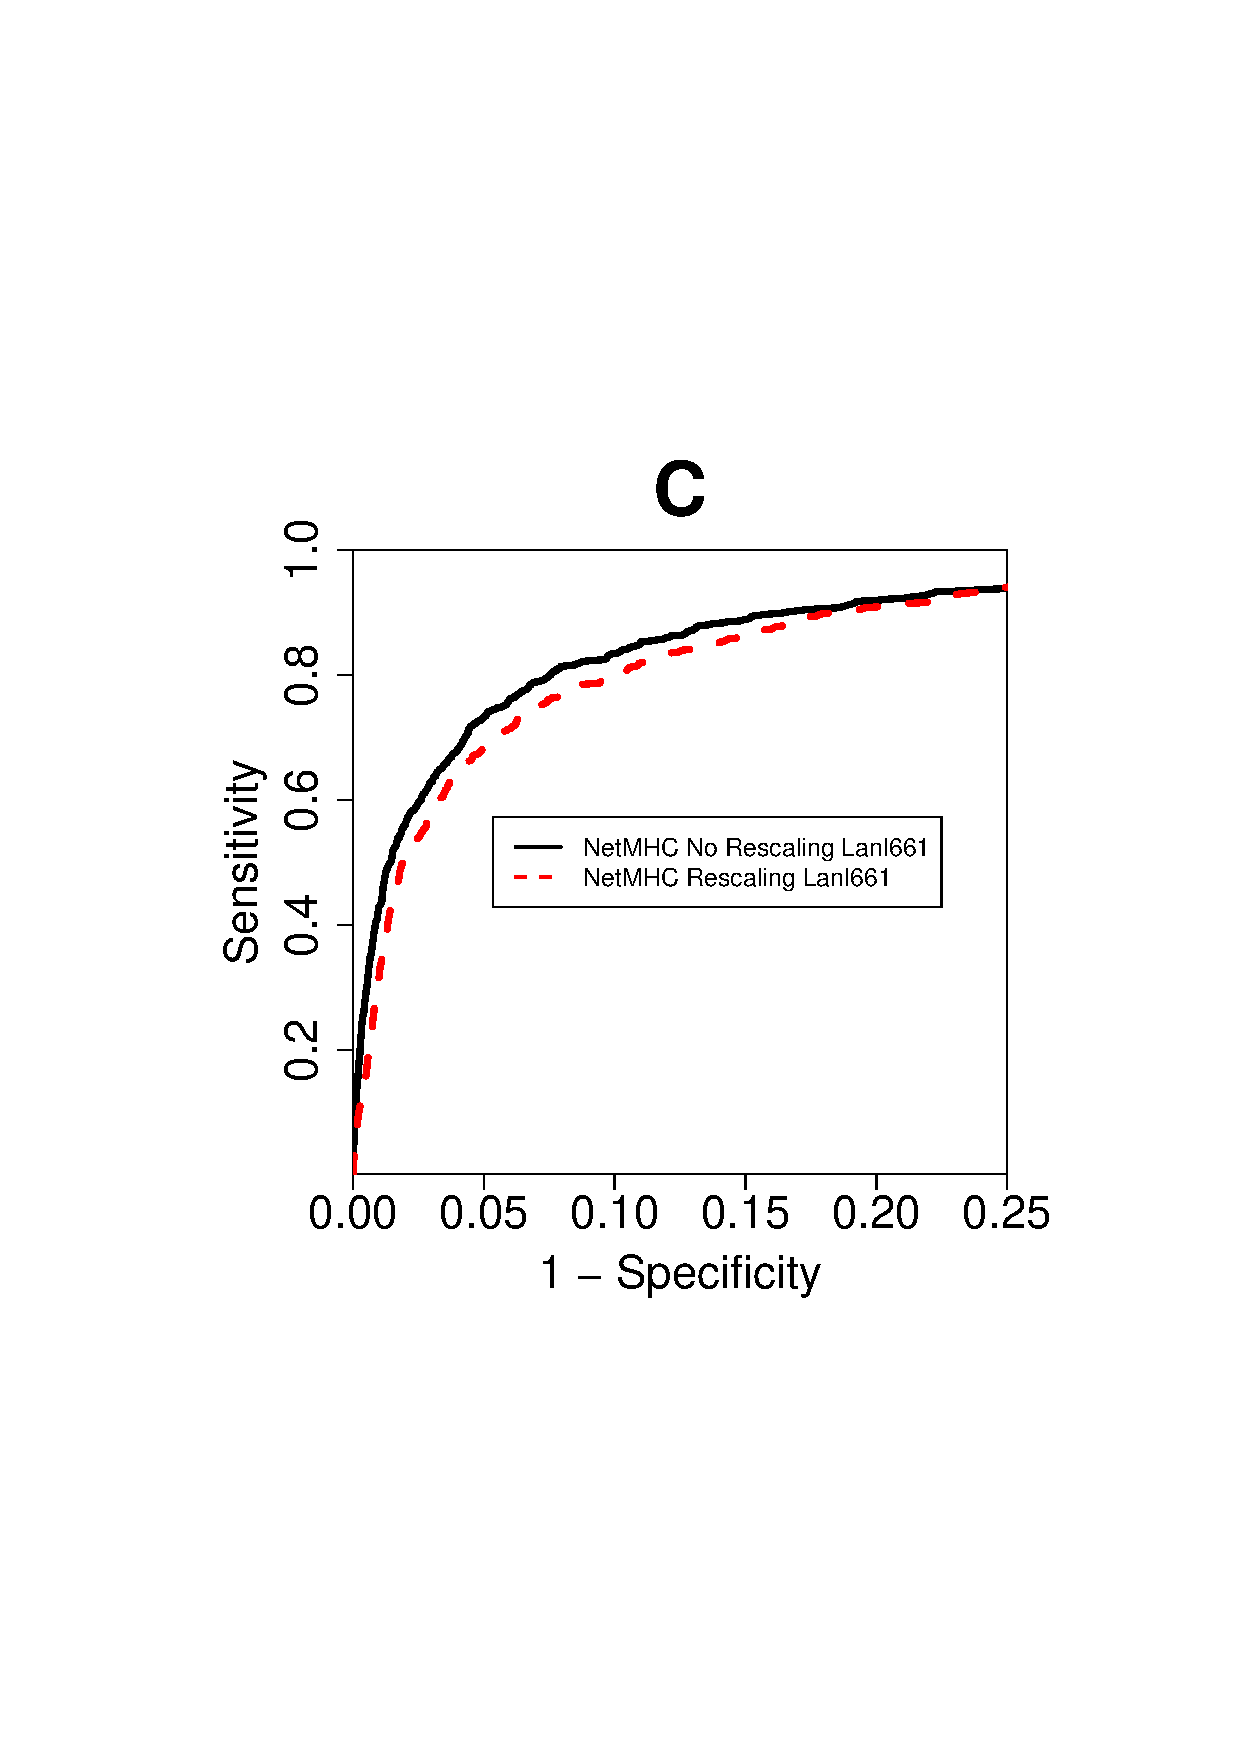
\includegraphics[width=7cm]{./Figures/chapter4/figure_1C}%
\hspace{0cm}%
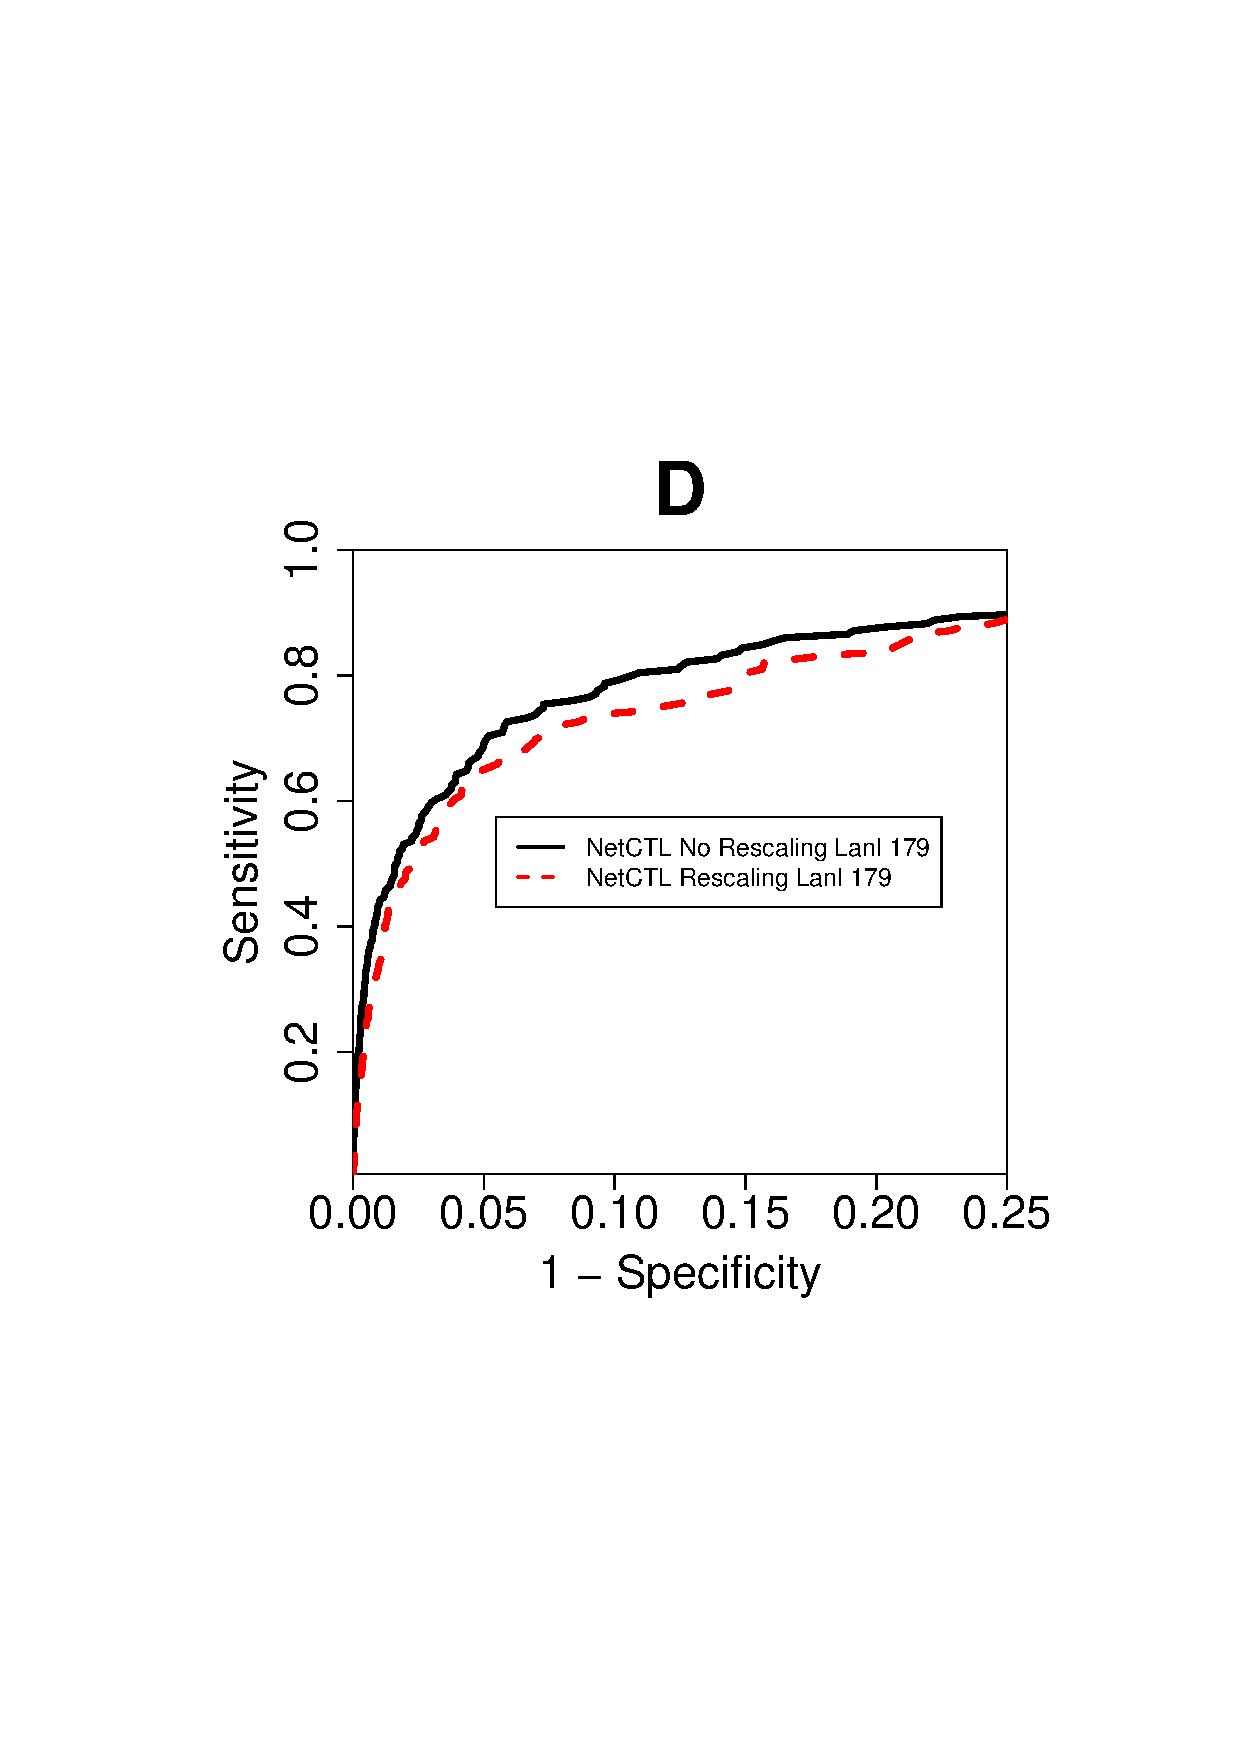
\includegraphics[width=7cm]{./Figures/chapter4/figure_1D} \\
\caption[The ROC curves comparing rescaling and non-rescaling]{Each graph shows the ROC curves using different combinations of datasets and prediction methods (see \tref{chapter4/table1}). A uses NetCTL with the SYF$^1$ dataset, B uses NetMHC with the SYF$^1$ dataset, C uses NetMHC with the Lanl$^{661}$ dataset and D uses NetCTL with the Lanl$^{179}$ dataset. The x-axis has been scaled to show the region of importance (the AUC with high specificity values). The rescaled results (red dashed line) are compared against non-rescaled (black solid line). \tref{chapter4/table1} gives the statistics for each graph.}
\label{chapter4/figure1}
\end{figure}

\subsection{Comparison of Rescale Values}

We calculated rescale values based on the predicted binding to 500,000 peptides selected at random from \emph{Mycobacterium tuberculosis}. To check that the source of the peptides did not alter our conclusions we randomly selected 500,000 natural peptides from the Swiss-Prot database \citep{Consortium2008} and produced the top percentile re-scaling values for each allele from these peptides. \fref{chapter4/rescaleValues} compares these values to the re-scaling values we previously used, which were derived from non-overlapping peptides from \emph{Mycobacterium tuberculosis}. As can be seen from \fref{chapter4/rescaleValues}, the two sets of rescale values are strongly positively correlated ($R^2 = 0.9563$, $P < 0.001$). Repeating our ROC curve analysis of rescaled and non-rescaled predictions from \fref{chapter4/figure1} C using these new rescale factors (\fref{chapter4/randomROC}) gives very similar results to those reported here. Consequently, whether we calculate the rescale factors using random natural peptides from \emph{Mycobacterium tuberculosis} or on random natural peptides from a range of proteins, our conclusions remain unchanged.

\begin{figure}[htp]
\centering
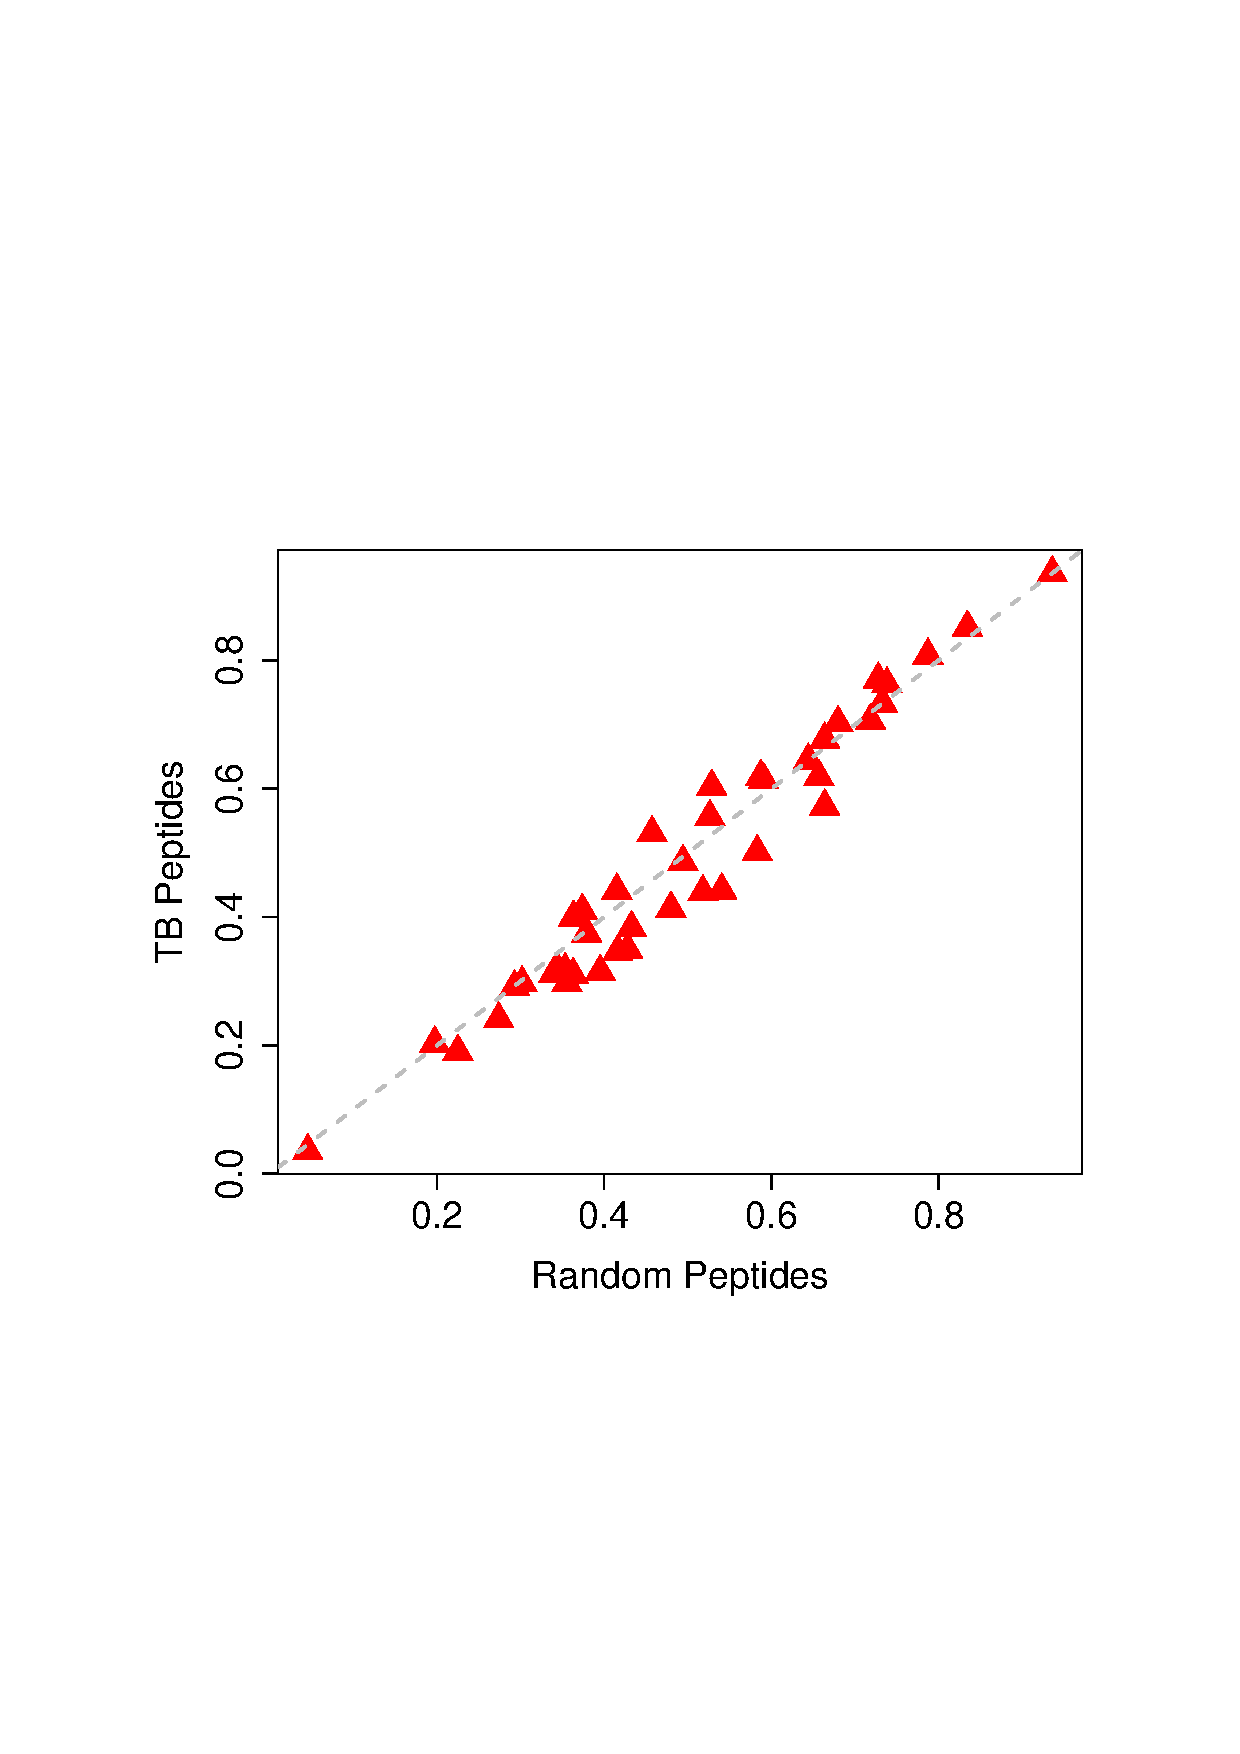
\includegraphics[width=14cm]{./Figures/chapter4/rescaleValues}
%\rule{35em}{0.5pt}
\caption[The relationship between rescale values]{The relationship for the top percentile rescaling values for each allele between random natural peptides and non-overlapping peptides from Mycobacterium tuberculosis. There was no significant difference between the two measures (Mann-Whitney paired test, $P = 0.1181$) and the data was strongly correlated ($R^2 = 0.9563$, $P < 0.001$).}
\label{chapter4/rescaleValues}
\end{figure}

\begin{figure}[htp]
\centering
\includegraphics[width=10cm]{./Figures/chapter4/randomROC}
%\rule{35em}{0.5pt}
\caption[The ROC curve analysis without with randomly derived rescale values]{The ROC analysis of the Lanl$^{661}$ dataset. The rescale values used are derived from random natural peptides, as opposed to peptides originating from \emph{Mycobacterium tuberculosis}. The difference remains significant between the two curves (bootstrap test: $P < 0.001$).}
\label{chapter4/randomROC}
\end{figure}

\subsection{Variation in Rescale Values as a Function of Accuracy}

One possible explanation for why rescaling has a detrimental impact on prediction is that there may be a positive correlation between rescale factor and allelic predictor accuracy (Morten Nielsen, pers.~comm.). To check this hypothesis we calculated the AUCs for each NetMHC v3.0 predictor using the Lanl$^{661}$ dataset and plotted this against the corresponding rescale factor, the results of which are shown in \fref{chapter4/figure2}. This shows no evidence of a correlation between rescaling values and the AUC values ($R^2 = 0.0068$, $P = 0.606$).

\begin{figure}[htp]
\centering
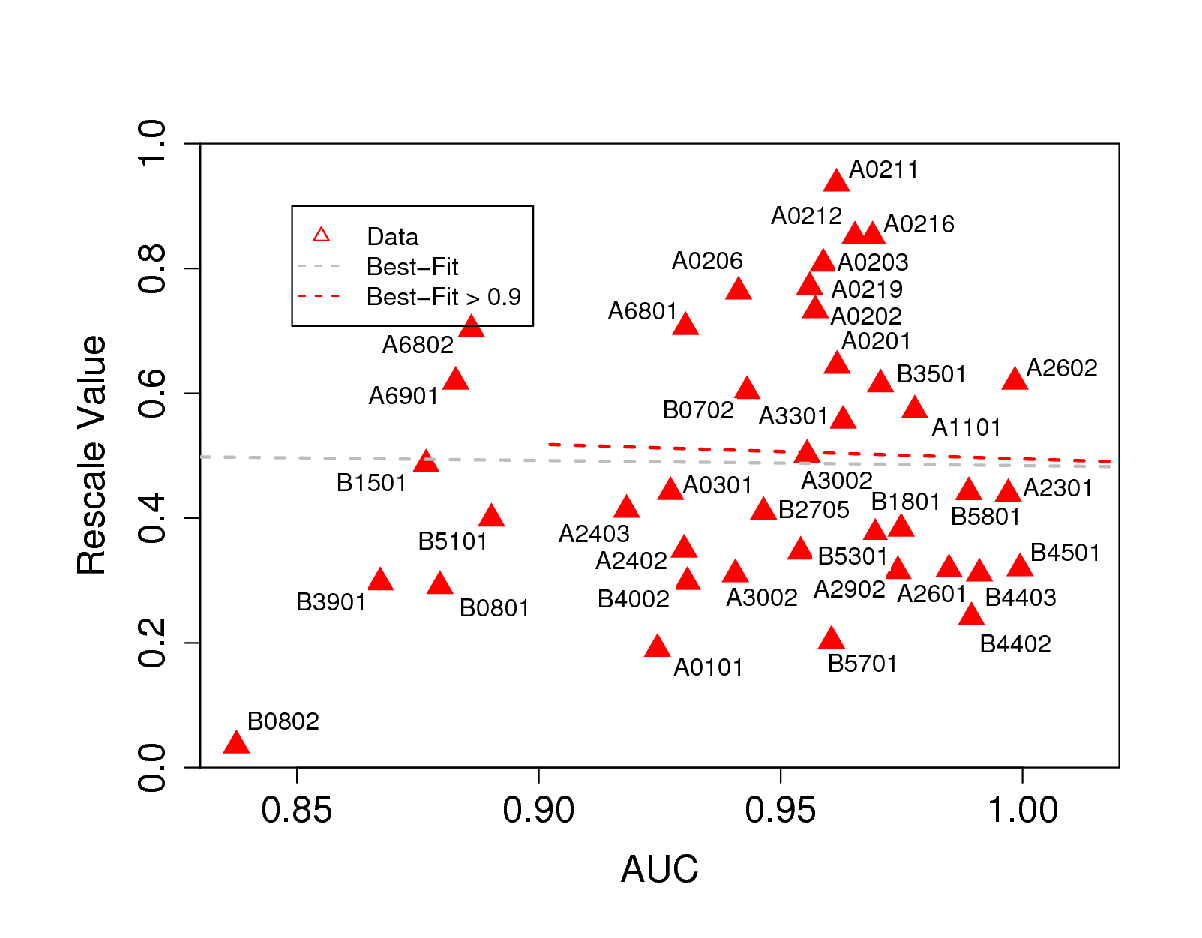
\includegraphics[width=14cm]{./Figures/chapter4/figure_2_edit_2}
%\rule{35em}{0.5pt}
\caption[The relationship between AUC and rescale value]{The relationship between AUC and rescale value. There is no evidence for a correlation of AUC and rescale value for the whole set of allele predictors ($R^2 = 0.0068$, $P = 0.606$), nor for the subset of predictors with an AUC $> 0.9$ ($R^2 = 0.0007$, $P = 0.887$). This analysis used the Lanl$^{661}$ epitope dataset.}
\label{chapter4/figure2}
\end{figure}

Consequently, it is unlikely that a correlation between rescale values and AUC values explains our findings. However, certain alleles like B0801 do have both a low rescale value and a low AUC. To double check that these poor accuracy predictors were not causing the inaccuracies in rescaled predictions we repeated our ROC curve analysis for Lanl$^{661}$ without the low accuracy predictors (those with an AUC value below 0.9; namely A6801, A6802, B3501, B0702, B0801, B0802 and B4501). In the remaining, reduced subset of predictors there was even less evidence for a correlation between AUC and rescale factor ($R^2 = 0.0007$, $P = 0.887$). For this subset of predictors the accuracy was still significantly better if rescaling was not applied (\fref{chapter4/reducedROC}; bootstrap test: $P < 0.001$) and comparable to the ROC curve analysis using the full set of alleles (\fref{chapter4/figure1} A).

Therefore, we believe there is no evidence to support the hypothesis that the reason rescaling is detrimental is because there is a correlation between rescale factors and AUC. 

\begin{figure}[htp]
\centering
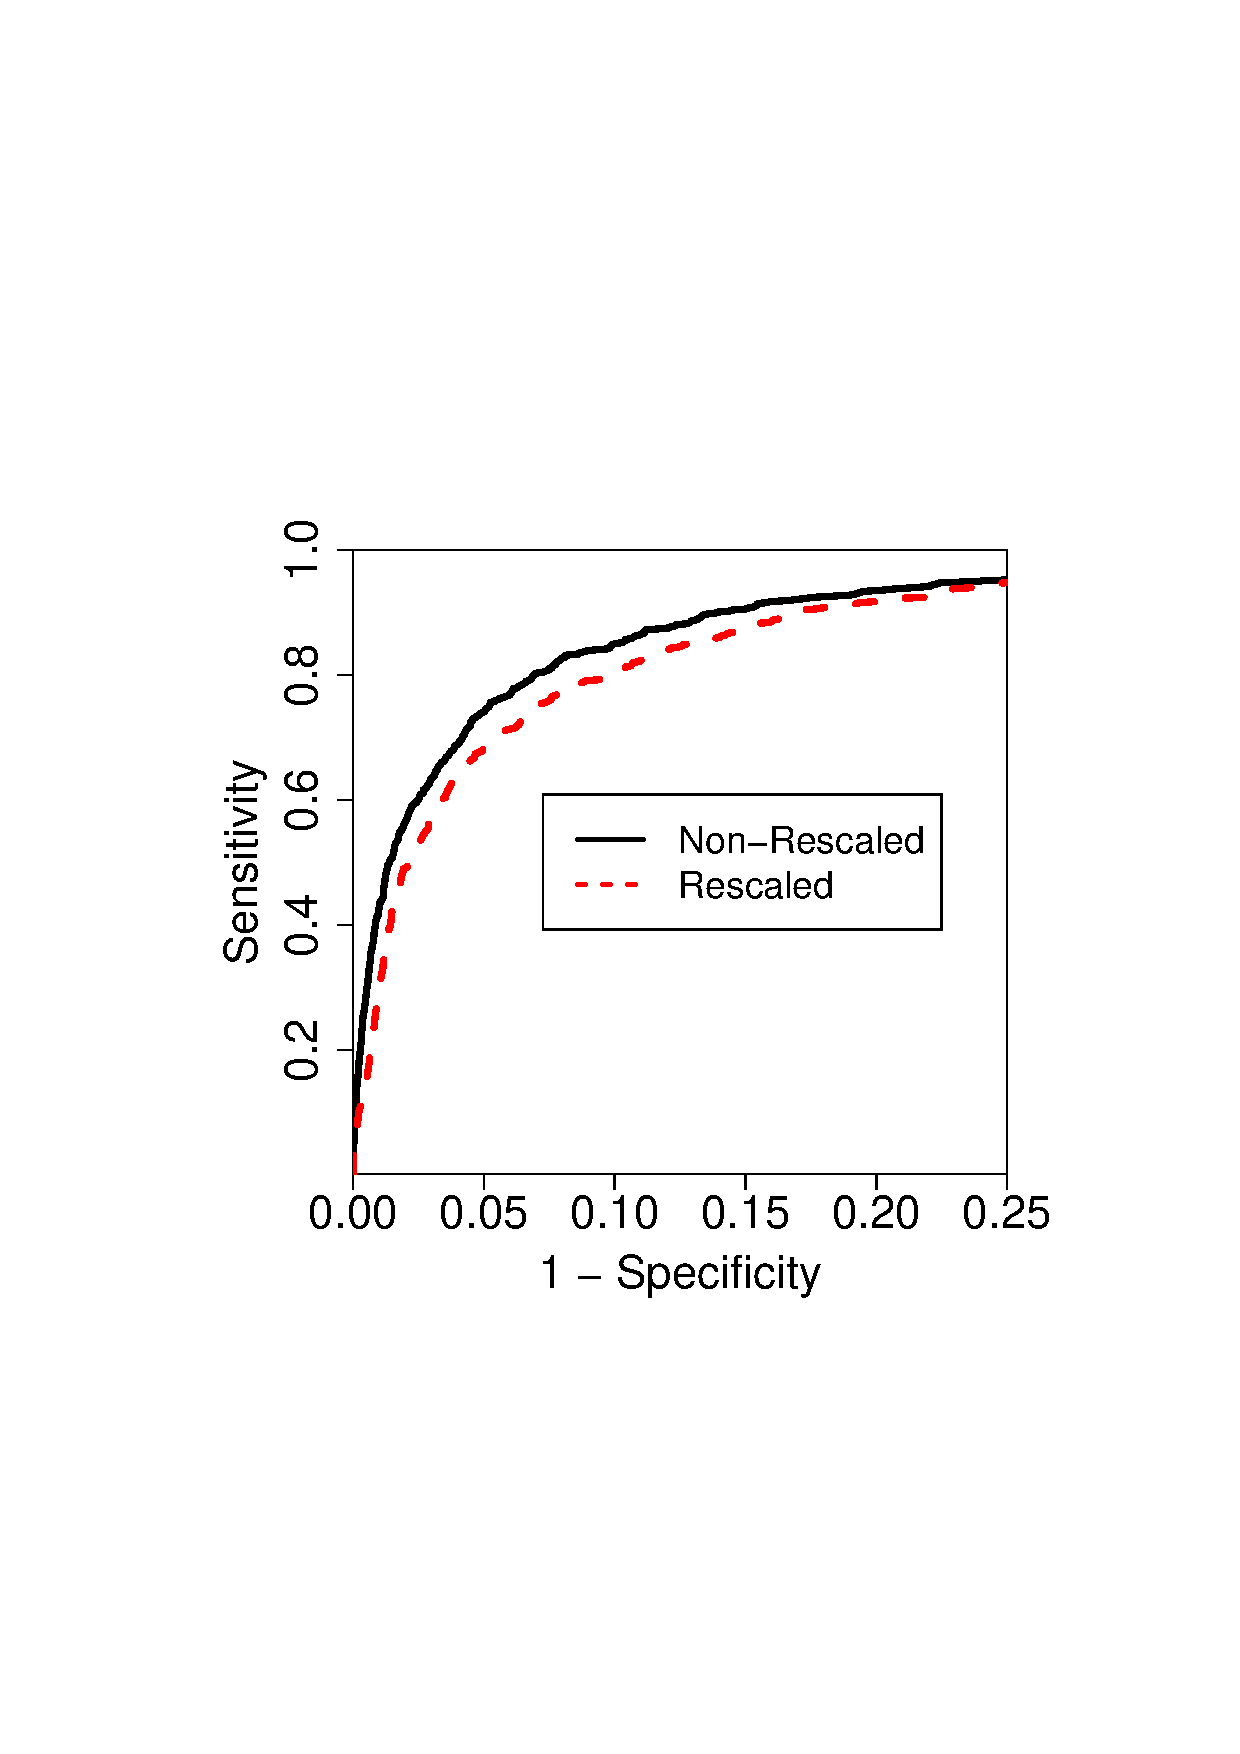
\includegraphics[width=10cm]{./Figures/chapter4/reducedROC}
%\rule{35em}{0.5pt}
\caption[The ROC curve analysis without low accuracy alleles]{The result of the ROC curve analysis, using the Lanl$^{661}$ dataset and excluding any alleles (7 in total) that had an AUC $< 0.9$ from \fref{chapter4/figureAffinityComp} (bootstrap: $P < 0.001$).}
\label{chapter4/reducedROC}
\end{figure}

\subsection{Other Measurements of Performance}

We used 3 other metrics \citep{larsen2007} to compare predictive performance with and without rescaling.

\begin{enumerate}
\item The rank of known epitopes was compared with non-epitopes from the same protein for both rescaled and non rescaled predictions. From \fref{chapter4/figureBoxplots}, it can be seen that the non-rescaled results produced significantly more accurate results for both epitope datasets (paired Wilcoxon ranked sum test, $P < 0.001$).

\begin{figure}[htp]
\centering
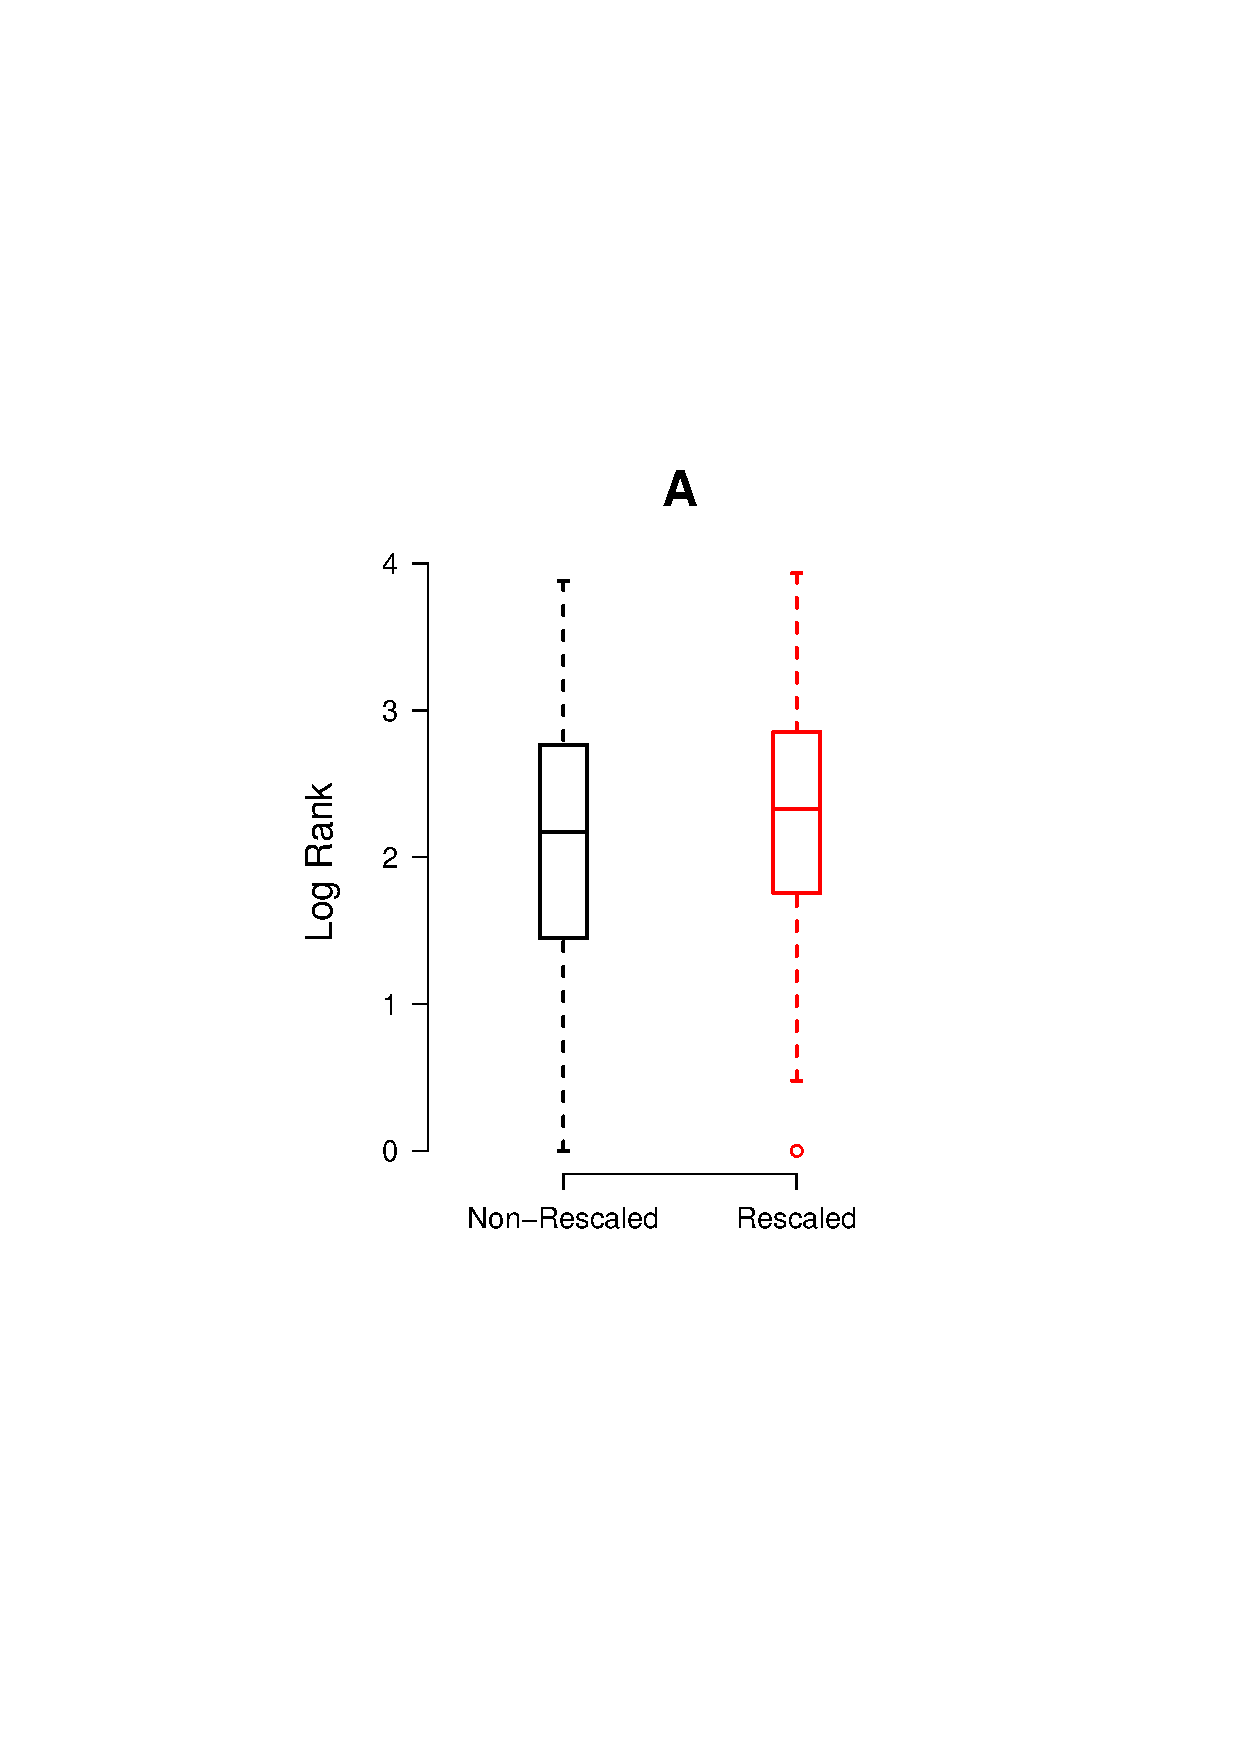
\includegraphics[width=7cm]{./Figures/chapter4/boxplotA}%
\hspace{0cm}%
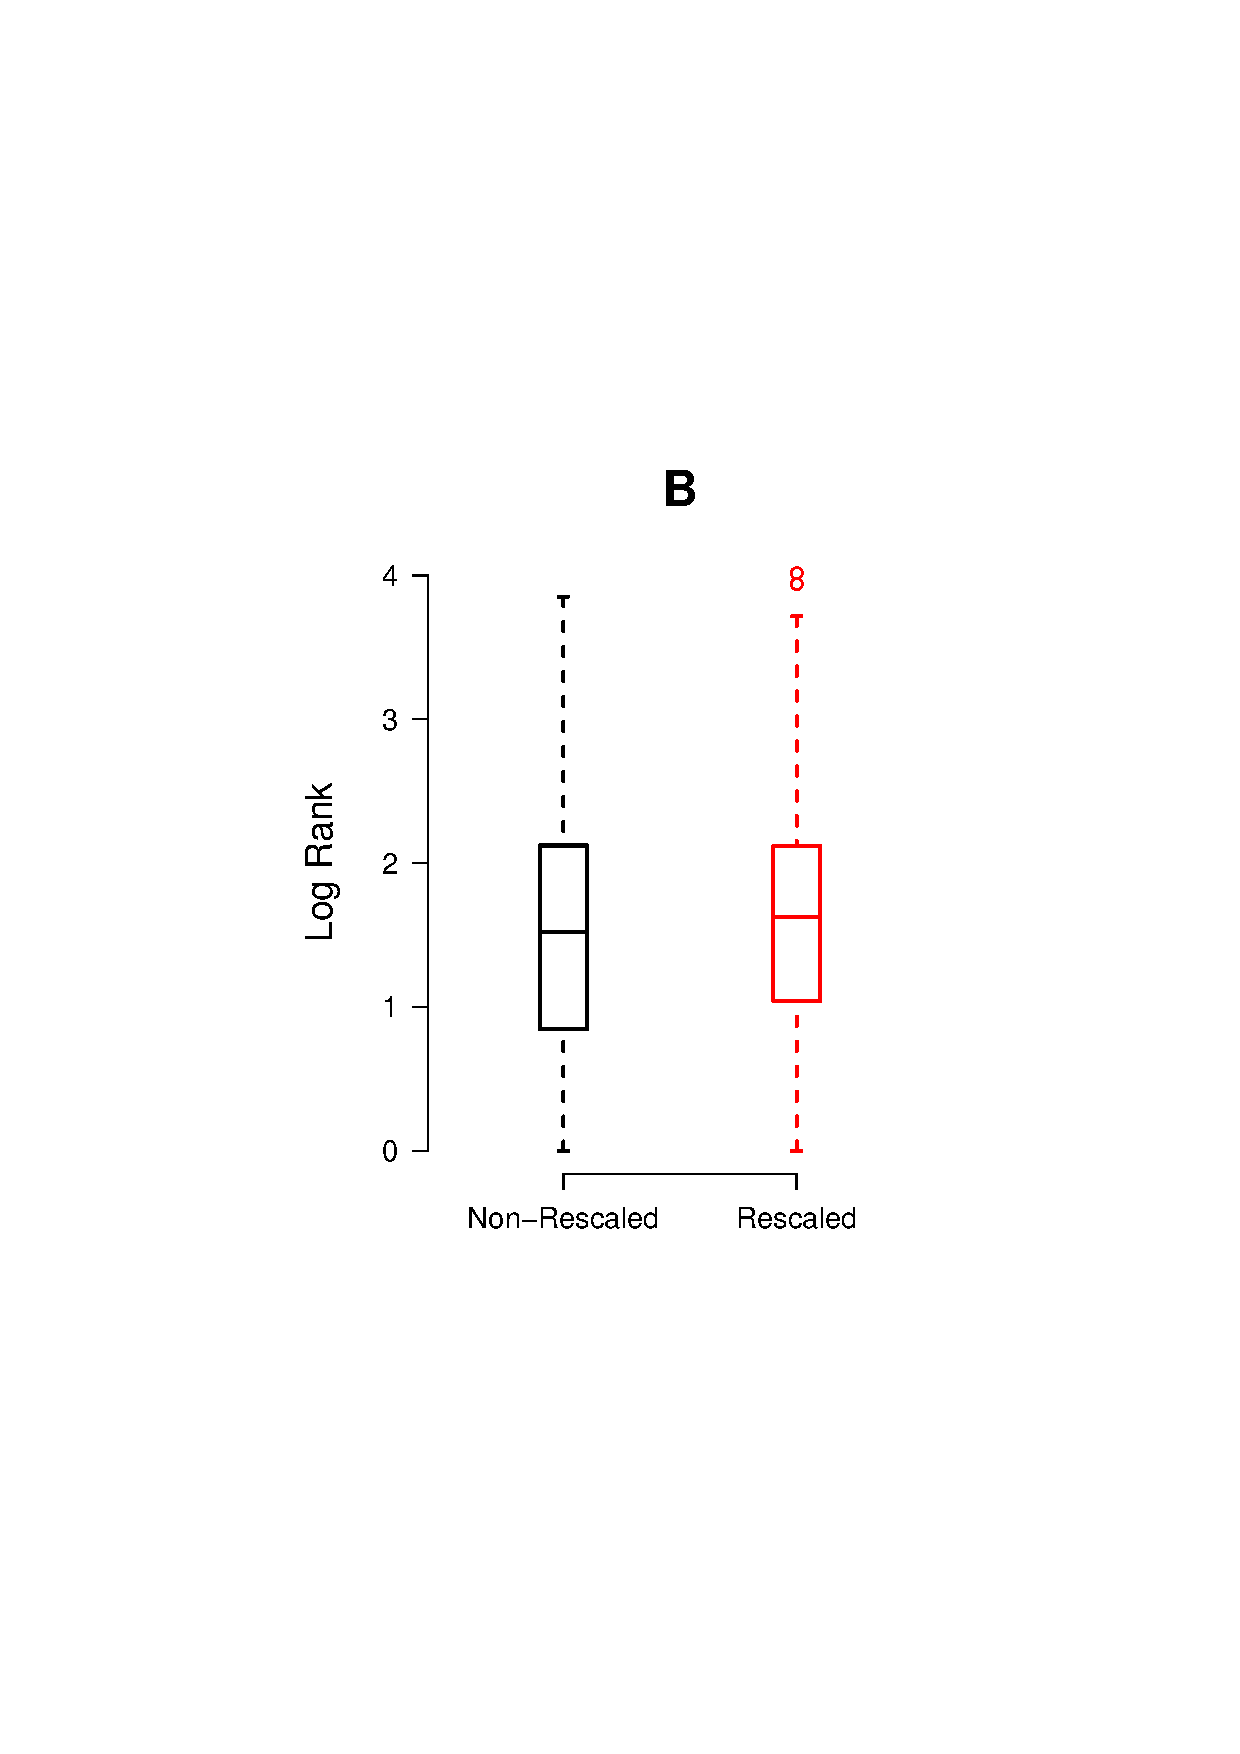
\includegraphics[width=7cm]{./Figures/chapter4/boxplotB} \\
\caption[]{\textbf{(A)} A box plot showing the summary statistics of the ranks ($\log_{10}$) of each of the 216 epitopes in the HIV dataset among all overlapping 9-mer in the epitopes' source proteins. The ranks of the epitopes were significantly lower for non-rescaled scores compared to rescaled scores (Paired Wilcoxon ranked sum test, $P < 0.001$). The non-rescaled scores produced a higher rank for 170 epitopes and rescaled scores for 24 epitopes. \textbf{(B)} The same analysis using 863 epitopes from the SYFPEITHI dataset. The ranks of the epitopes were significantly lower for non-rescaled scores compared to rescaled scores (Paired Wilcoxon ranked sum test, $P < 0.001$). The non-rescaled scores produced a higher rank for 474 epitopes and rescaled scores for 369 epitopes.}
\label{chapter4/figureBoxplots}
\end{figure}

\item Predicted binding affinities that had not been rescaled produced improved results compared to predictions that had been rescaled at given sensitivities using the epitope datasets from \citep{larsen2007} (\tref{chapter4/table2}).

\begin{table}[htp]
\begin{center}
\begin{tabular}{|c|c|c|c|}
\hline
Sensitivity & No Rescaling & Rescaling & Epitope Set \bigstrut \\
\hline
0.3 & 0.995 & 0.989 & \multirow{3}{*}{HIV$^{216}$} \bigstrut[t] \\
0.6 & 0.987 & 0.977 & \\ 
0.8 & 0.921 & 0.891 & \bigstrut[b] \\
\hline
0.3 & 0.998 & 0.997 & \multirow{3}{*}{SYF$^{863}$} \bigstrut[t] \\
0.6 & 0.991 & 0.991 & \\ 
0.8 & 0.974 & 0.973 & \bigstrut[b] \\ 
\hline
\end{tabular}
\end{center}
\caption[Specificity at specified sensitivity values]{The specificity of non-rescaled and rescaled results at specified sensitivity values. Epitope datasets are taken from \citep{larsen2007}.}\label{chapter4/table2}
\end{table}

\item Predicted binding affinities that had not been rescaled also showed an improvement over rescaled affinities when comparing the total number of true epitopes found among the top 5\% of peptides predicted to bind (\tref{chapter4/table3}), again using the epitope datasets from \citep{larsen2007}.

\begin{table}[htp]
\begin{center}
\begin{tabular}{|c|cc|}
\hline
Epitope Set & No Rescaling & Rescaling \bigstrut \\
\hline
SYF$^{863}$ & 0.885 & 0.877 \bigstrut[t] \\
HIV$^{216}$ & 0.718 & 0.690 \bigstrut[b] \\
\hline
\end{tabular}
\end{center}
\caption[The top 5\% of predicted binding affinities]{The fraction of the total number of epitopes in the 2 epitope datasets among the top 5\% of predicted binding affinities.}\label{chapter4/table3}
\end{table}

\end{enumerate}

\subsection{The Effect of Rescaling on Quantitative Predictions of Binding Affinities}
Using 2 sets of experimentally-derived epitope-allele binding affinities, we also showed that the correlation between predicted and experimental affinities was weaker with rescaling than without.

A set of 128 experimentally-derived epitope-allele binding affinities was extracted from the Immune Epitope Database and Analysis Resource \citep{peters2005}. This set of epitopes was known to have no involvement in the training of any of the allelic predictors in NetMHC v3.0 or NetCTL v1.2.

The relationship between the rescaled / non-rescaled predicted binding affinities and the experimental binding affinities was investigated (\fref{chapter4/figureAffinityComp}). Rescaling resulted in a significantly larger error (the difference between predicted and experimental affinity) compared to predicted binding affinities that were not rescaled ($P < 0.001$). Although rescaling would naturally result in a larger quantitative error, additionally, the correlation between predicted and experimental affinities was weaker with rescaling than without (rescaled: $P < 0.001$, Spearman's $\rho = 0.40$; not rescaled: $P < 0.001$, Spearman's $\rho = 0.51$).

The analysis was repeated using a second experimental dataset. This second dataset came from the Sette and Buus laboratories and included the experimental data used to train NetMHC and NetCTL. The results obtained using this second dataset were very similar to those obtained using the first, independent dataset (\fref{chapter4/figureCompareAll}).

\begin{figure}[htp]
\centering
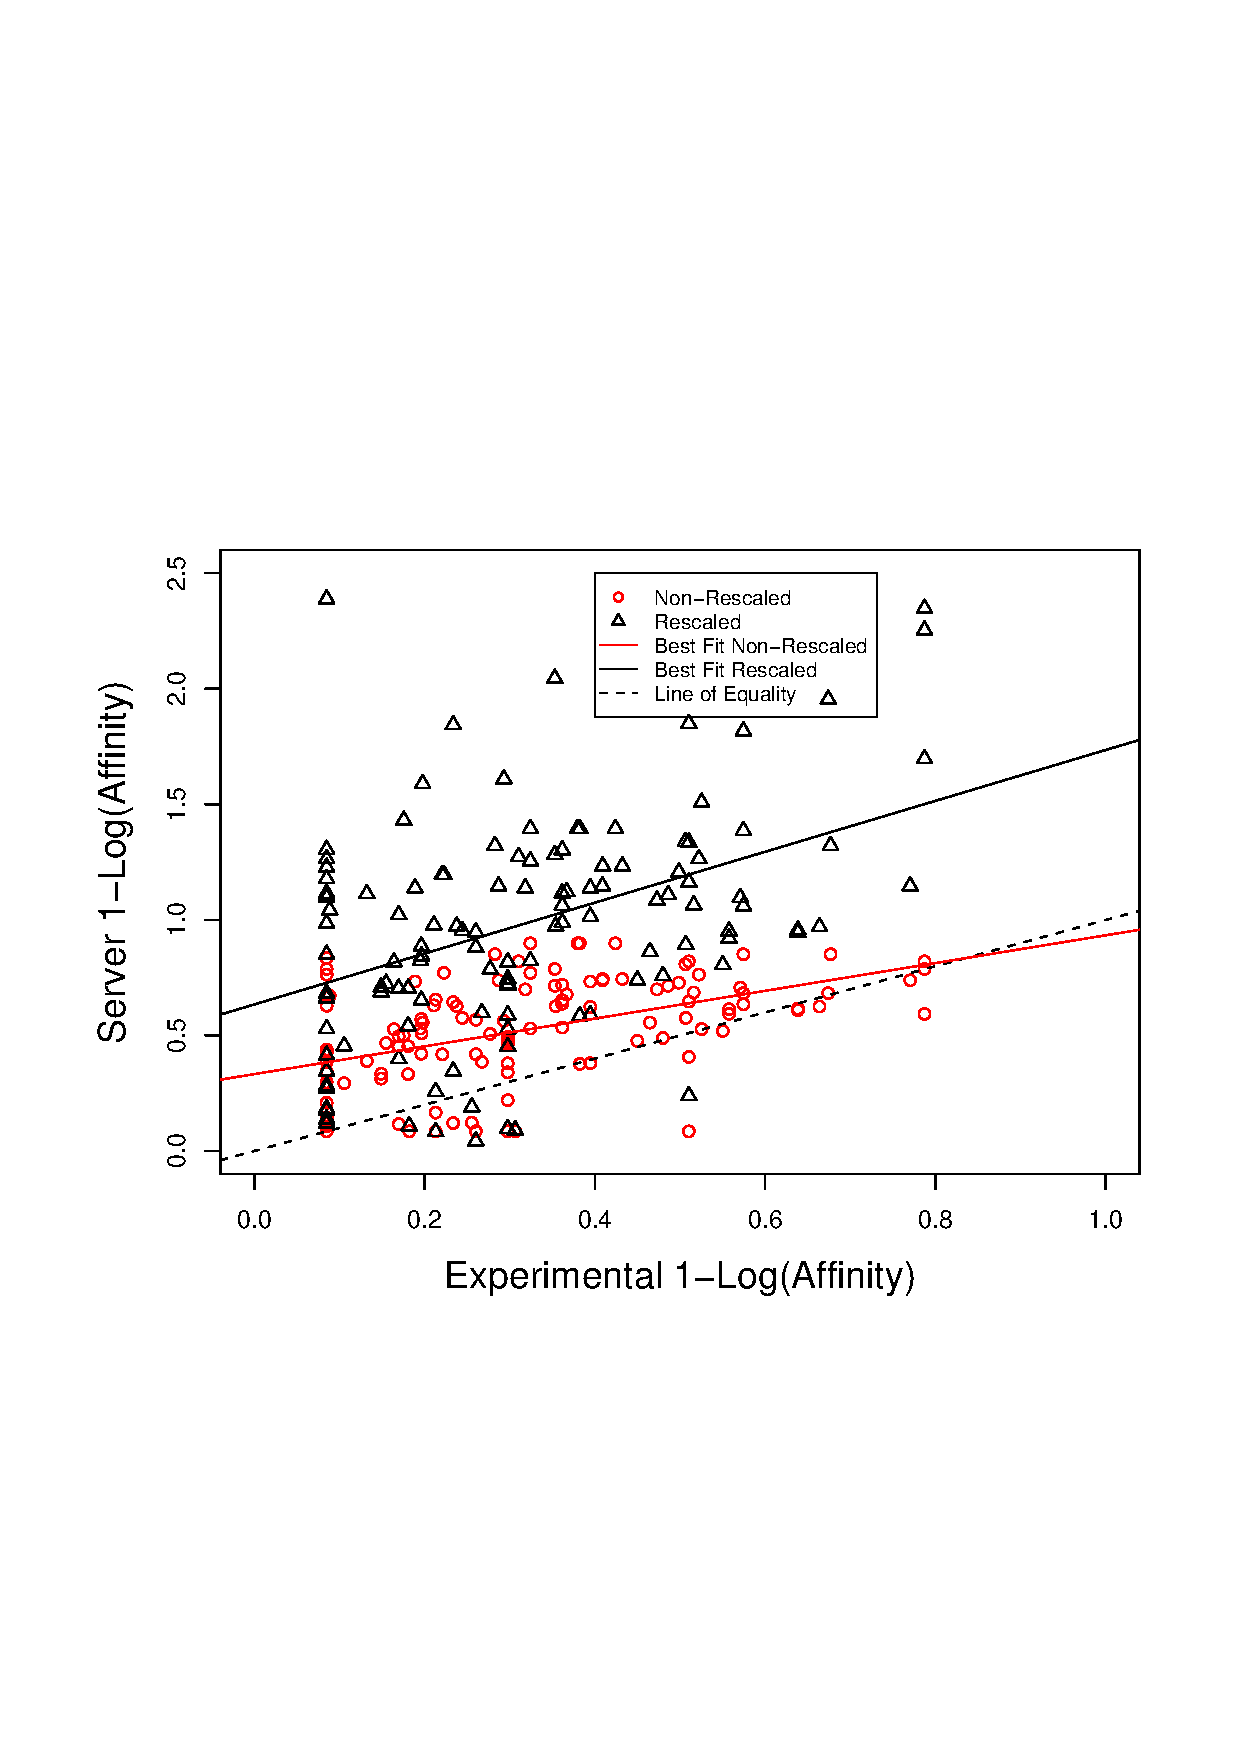
\includegraphics[width=14cm]{./Figures/chapter4/figureAffinityComp}
%\rule{35em}{0.5pt}
\caption[A comparison of experimental and predicted binding affinities]{The experimental binding affinities for 128 epitopes were obtained from IEDB \citep{peters2005} and converted to a log scale ($1-\log _{50000} \left( \text{affinity} \right)$). These epitopes were then tested using NetMHC v3.0 to produce 2 sets of predicted binding affinities; rescaled or non-rescaled. The predicted scores were also converted to a log scale ($1-\log _{50000} \left( \text{affinity} \right)$) and the non-parametric Spearman's $\rho$ was used to calculate the correlation between experimental and predicted data.}
\label{chapter4/figureAffinityComp}
\end{figure}

\begin{figure}[htp]
\centering
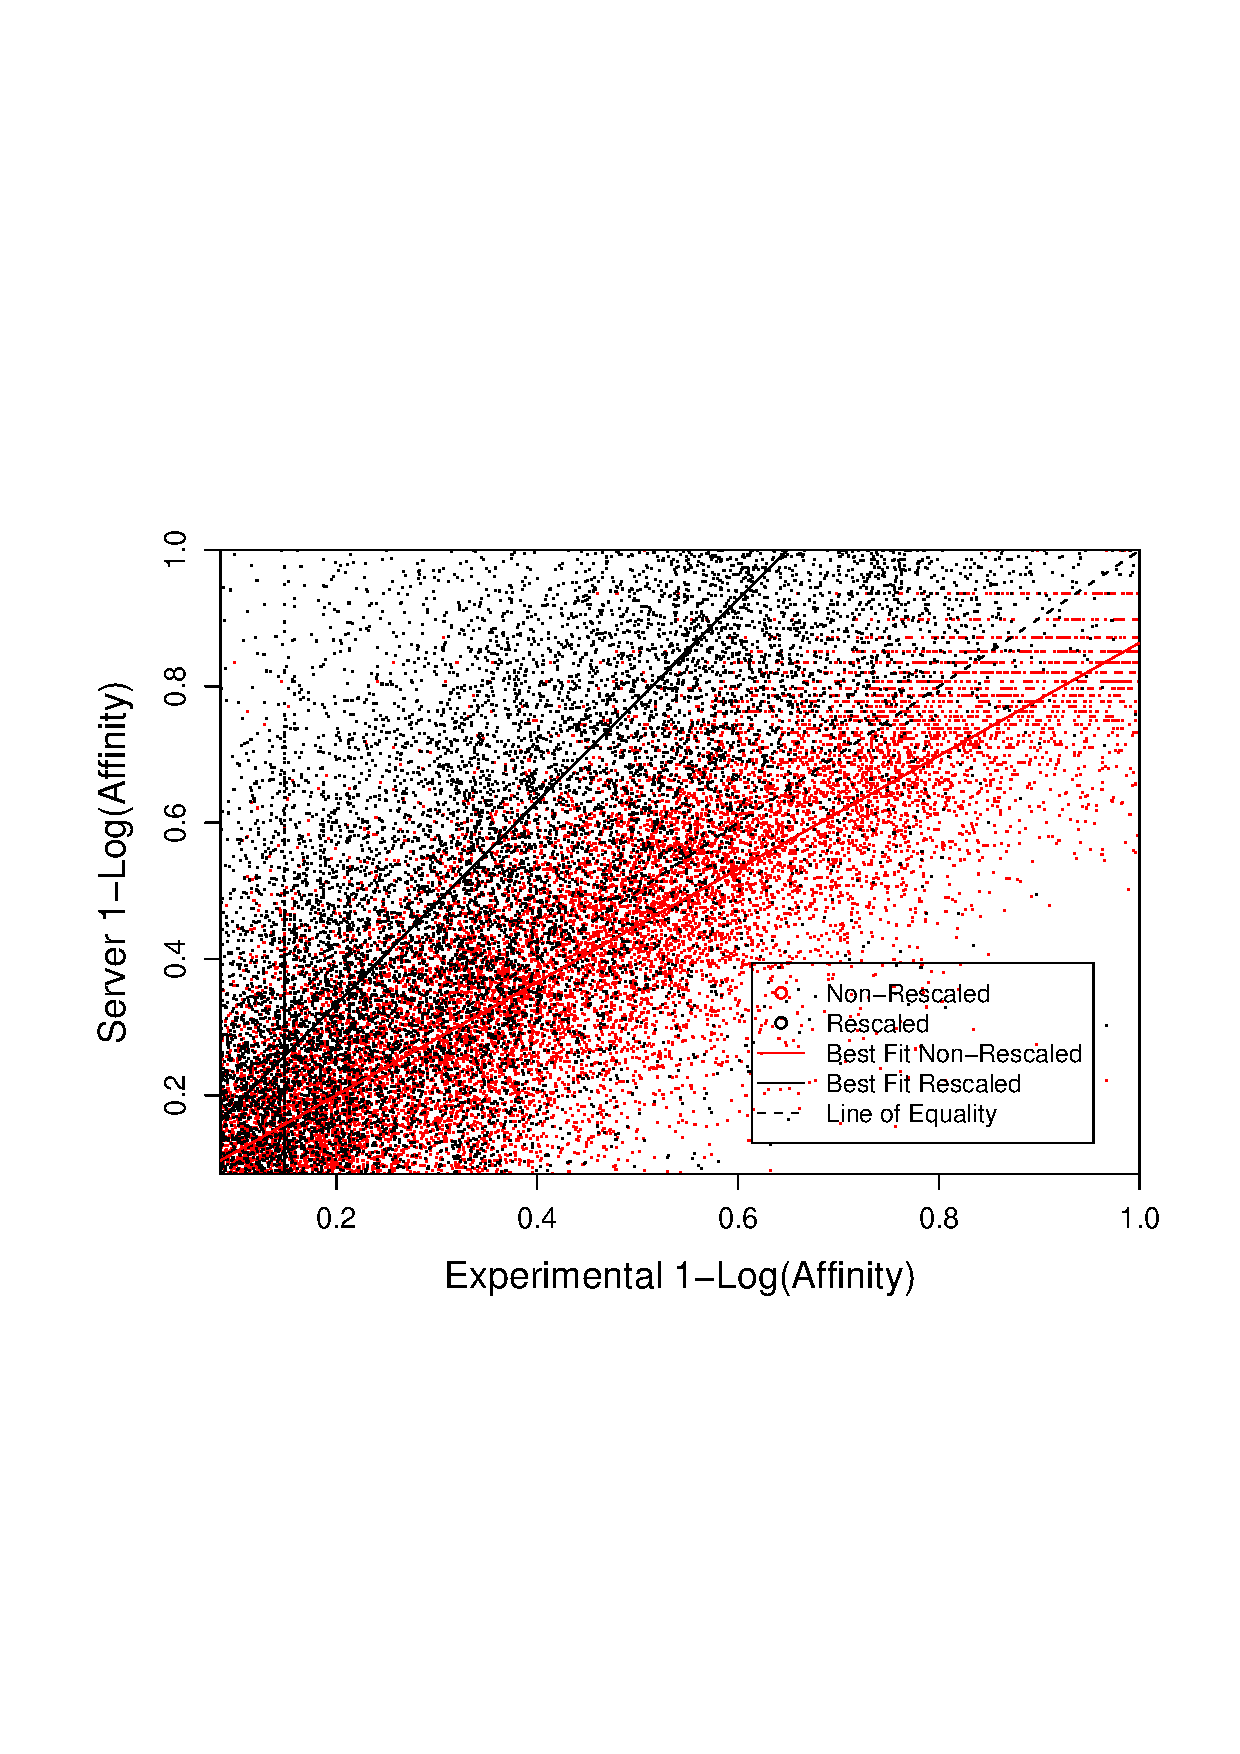
\includegraphics[width=14cm]{./Figures/chapter4/figureCompareAll}
%\rule{35em}{0.5pt}
\caption[A second comparison of experimental and predicted binding affinities]{The experimental binding affinities for 29,336 epitopes were obtained from IEDB and converted to a log scale ($1-\log _{50000} \left( \text{affinity} \right)$). These epitopes were then tested using NetMHC v3.0 to produce 2 sets of predicted binding affinities; rescaled or non-rescaled. The predicted scores were also converted to a log scale ($1-\log _{50000} \left( \text{affinity} \right)$) and the non-parametric Spearman's $\rho$ was used to calculate the correlation between experimental and predicted data. The correlation between non-rescaled predicted affinities and experimental data showed a $P$ value of $< 0.001$ (Spearman's $\rho$ = 0.877). Rescaled predicted affinities and experimental data gave a $P$ value of $< 0.001$ (Spearman�s $\rho$ = 0.816). The absolute difference between the 2 best-fit lines and the line of equality was calculated and it was shown that the non-rescaled values were significantly closer to the line of equality (Wilcoxon Paired Signed Rank Test; $P$ value $< 0.001$).}
\label{chapter4/figureCompareAll}
\end{figure}

\subsection{The Effect of Negative Data Volume}\label{chapter4/results/NegVol}

As explained in \sref{chapter4/methodsDatasets}, we multiplied the negative set of each dataset by the number of allele predictors being tested. This was to mirror an analysis where one would check every possible peptide-allele pair of a pathogen-MHC class I interaction when searching for potential epitopes. A possible argument was that the resultant positive/negative ratio in our datasets was unrealistically low with such a high proportion of negative data. To counter this, the SYF$^1$ dataset was modified to contain 148 positive epitopes and 78,111 negative peptides, which gave a positive/negative ratio of 0.2\%, a figure close to the estimated 1\% of all natural peptides that would bind to a given MHC molecule \citep{larsen2005}. In order to test the difference in prediction accuracy between rescaled and non-rescaled predicted affinities with this reduced dataset, each of the 78,111 negative peptides was randomly paired with 1 of the 10 supertype predictors (see \sref{chapter4/methodsSYF1}) and the predicted binding affinity was found for each of theses pairs. Rescaling again resulted in a significant loss of performance (bootstrap test: $P < 0.001$, \fref{chapter4/figureReducedNeg}).

Related to this result, we performed a general analysis of the effect of positive and negative set size on the AUC values obtained in ROC curve analysis. As this is outside the scope of this chapter, this is explained in \aref{AppendixA/sizeEffects}.

\begin{figure}[htp]
\centering
\includegraphics[width=12cm]{./Figures/chapter4/figureReducedNegative}
\caption[The effect of a reduced negative dataset]{The result of the ROC curve analysis, using the SYF$^1$ dataset, with a negative set of 78,111 peptides. The difference remains significant between the two curves (bootstrap test: $P < 0.001$).}
\label{chapter4/figureReducedNeg}
\end{figure}

\subsection{Is Rescaling Necessary to Maintain Low Variation in Sensitivity?}

Another argument that could be made for rescaling is that, in its absence, those allele predictors with a lower accuracy would have lower sensitivity i.e.~fewer epitopes would be detected from those particular alleles (Morten Nielsen, pers.~comm.). We tested this hypothesis using the SYF$^1$ dataset. A score threshold value for rescaled and non-rescaled affinity values was identified at a specificity of 0.95 for the complete dataset (0.2068 for non-rescaled affinity values and 0.4330 for rescaled affinity values, using $1-\log _{50000} \left( \text{affinity} \right)$). Next the sensitivity and specificity values per supertype allele were calculated at these threshold values. The result is shown in \fref{chapter4/figureRevArg}. There is no evidence for a large decrease in the variation in allelic sensitivity upon rescaling. The ranges of sensitivities are identical with or without rescaling and the standard deviations are very similar (0.1526 non-rescaled, 0.1528 rescaled), if anything, slightly higher upon rescaling.

\begin{figure}[htp]
\centering
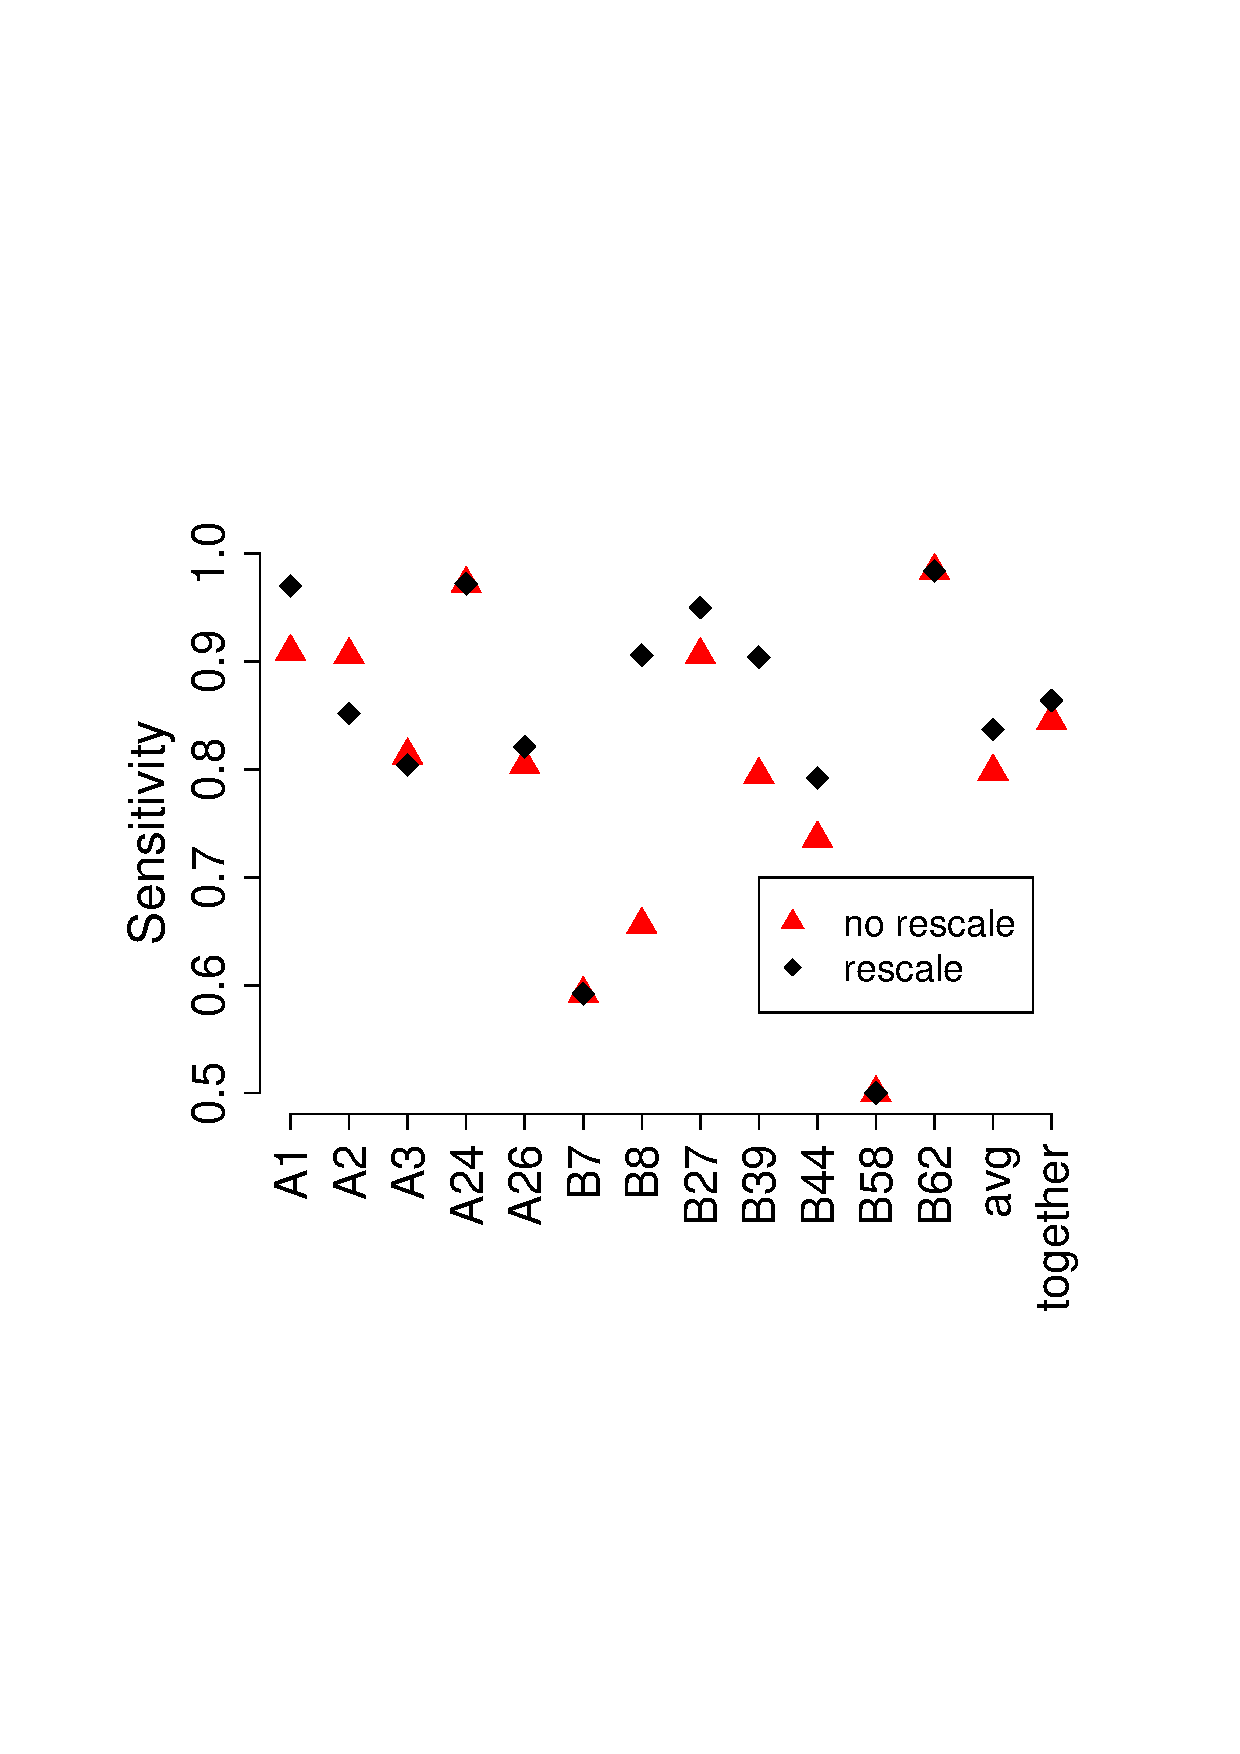
\includegraphics[width=12cm]{./Figures/chapter4/figureRevArg}
\caption[The effect of rescaling on sensitivity]{The effect of rescaling on sensitivity. For each supertype, the sensitivity was calculated when rescaling and not rescaling the predicted binding affinities. The final two results give the average sensitivities across all supertypes (`avg') and the sensitivities of all supertypes measured together (`together').}
\label{chapter4/figureRevArg}
\end{figure}

%%%%%%%%%%%%%%%%%%%%%%%%%%%%%%%%%%%%%%%%%%%%%%%%%%%%%%%%%%%%%%%%%%%%%%%%%%%%%%%%%%%%%%%%%%%%%%%%%%%%

\section{Producing Metaserver}\label{chapter4/results/metaserver}

These results demonstrated a significant improvement in accuracy over NetMHC v3.0 and NetCTL v2.1 when classifying epitopes across a number of HLA class I alleles. Therefor, we decided to produce our own web-based prediction server based on these results, which we called Metaserver.

Metaserver is summarised in \eref{chapter4/equation1}. In this calculation the NetMHC estimated binding affinity is still combined with a rescale value in order to take advantage of the NetCTL-specific information relating to the processing (TAP and cleavage) of the peptide before it binds to HLA class I. However, the rescale value for Metaserver is the same across all alleles and is an average of the rescale values for each individual allele. In summary, Metaserver takes binding information from NetMHC, TAP and cleavage information from NetCTL, but removes the assumption that each HLA class I binds the same number of peptides by `averaging out' the rescaling of the predicted binding affinity. 

\begin{align}
\text{Metaserver Epitope Score} =& \text{ NetMHC Binding Affinity} / \text{~`Averaged' Rescale Value } + \nonumber \\
& \; w_{1} * \text{NetCTL TAP} + w_{2} * \text{NetCTL Cleavage}
\label{chapter4/equation1}
\end{align}

\noindent
$w_1$ and $w_2$ above represent the weightings that are applied to the TAP and cleavage prediction scores respectively. In all calculations, $w_1 = 0.05$ and $w_2 = 0.15$. Metaserver uses a Perl LWP script to access the web servers NetMHC and NetCTL and the website itself is written in PHP (\fref{chapter4/websiteView}). 

\begin{figure}[htp]
\centering
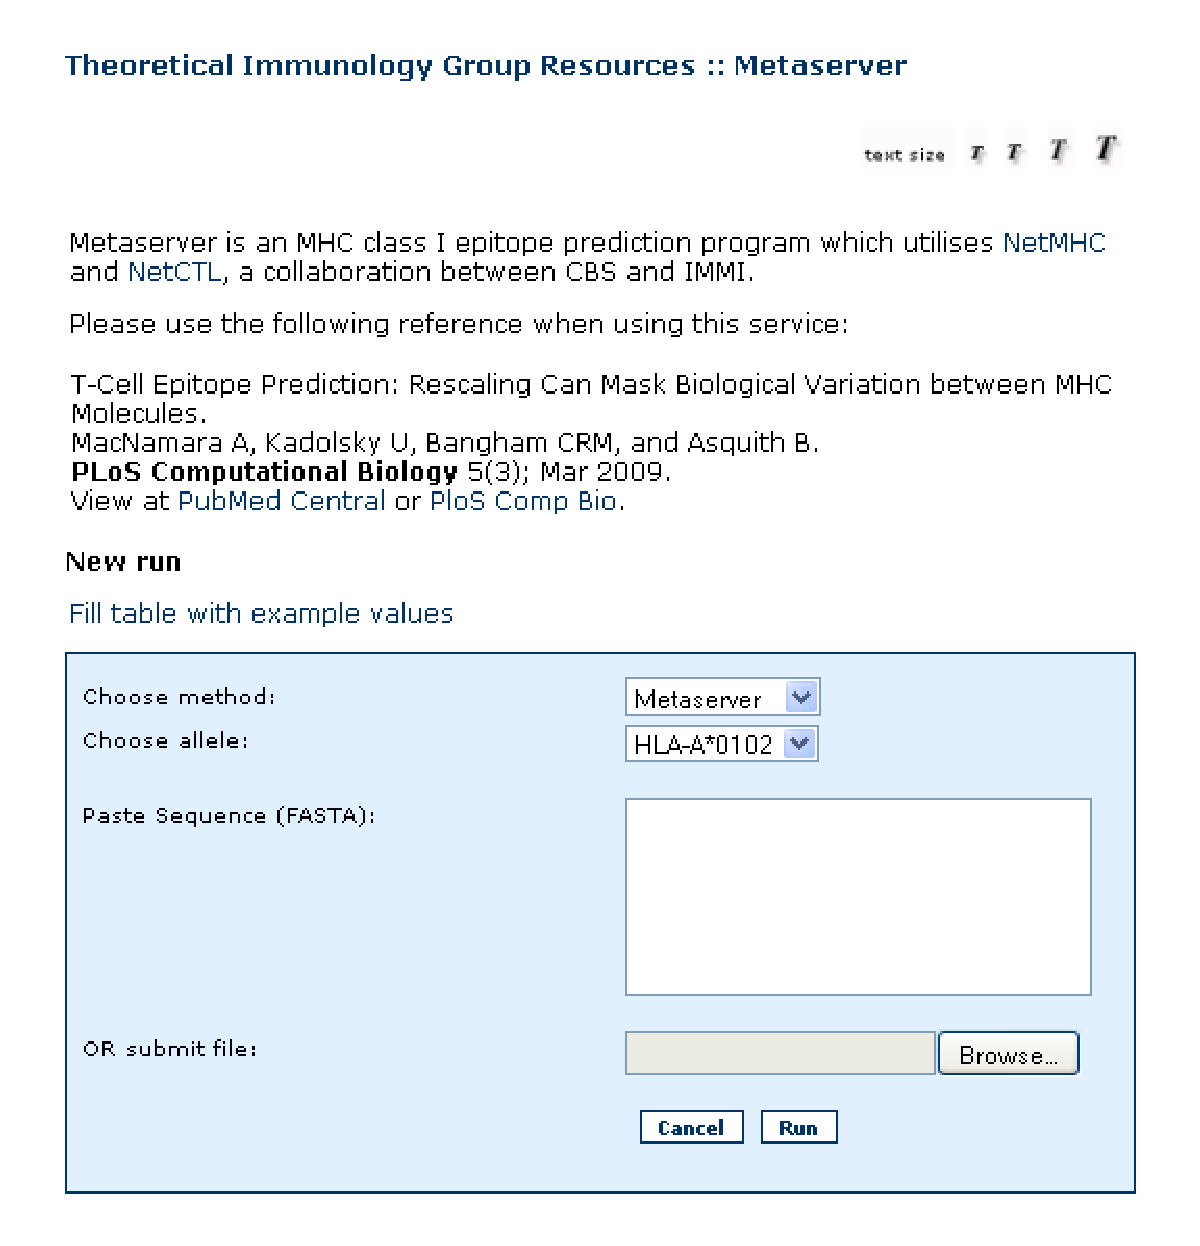
\includegraphics[width=10cm]{./Figures/chapter4/websiteView}
%\rule{35em}{0.5pt}
\caption[The Metaserver website]{A screenshot showing the Metaserver web-based resource. The site is hosted at:\\ \href{http://linuxwebdev.cc.ic.ac.uk/theoreticalimmunology/trans/metaserver.php}{\texttt{http://linuxwebdev.cc.ic.ac.uk/theoreticalimmunology/trans/metaserver.php}}\\}
\label{chapter4/websiteView}
\end{figure}

%%%%%%%%%%%%%%%%%%%%%%%%%%%%%%%%%%%%%%%%%%%%%%%%%%%%%%%%%%%%%%%%%%%%%%%%%%%%%%%%%%%%%%%%%%%%%%%%%%%%

\section{Discussion}

Rescaling is, in theory, a sound approach to improving epitope prediction and in particular comparability of predictions obtained using different allelic predictors. However, using a number of different measures of accuracy, in the context of two commonly used prediction methods, we have demonstrated that rescaling actually impairs rather than improves predictive performance and comparability. We suggest that rescaling predicted affinities results in a loss of information that outweighs any advantage gained in correcting for differences in training data. 

The first approach used ROC curve analysis and showed clear differences between rescaling and non-rescaling. The ROC curve gives a graphical representation of how well the prediction method ranks true epitopes among a set of non-binding peptides. Or to use an analogy, how efficient it is at finding the epitopic needle in a haystack of random peptides. From \fref{chapter4/figure1}, it is clear that rescaling across all allelic predictors results in a performance loss in terms of how well the method ranks its peptides by binding affinity; that is, rescaling impairs intra-allelic comparisons. This loss could be demonstrated using epitope data from a number of sources (SYFPEITHI, the HIV Molecular Immunology Database) and with two different methods of prediction (the combined approach of NetCTL v1.2 and NetMHC v3.0). This effect of rescaling would be detrimental to any studies screening across a number of alleles for possible epitopes (such as \citep{wang2007}). The effect of this performance difference can be gauged from \fref{chapter4/figure1} A. In order to identify correctly 85\% of the epitopes the percentage of false positives detected was 9\% and 15\%, for non-rescaled and rescaled methods respectively. To put this result into context, the viral protein NS1 from the H5N1 strain of Avian Influenza A consists of 221 overlapping nonamers. To screen this protein for potential epitopes, 33 epitopes would need to be experimentally checked for each MHC molecule of interest if rescaled predictions were used, as opposed to 20 for the non-rescaled predictions (providing 85\% epitope coverage was sufficient).

Added to the significant results from the ROC curve analysis, we also demonstrated the positive effect of removing rescaling in terms of the correlation with experimental data (\fref{chapter4/figureAffinityComp}) and also in terms of per-protein and sensitivity analysis (\fref{chapter4/figureBoxplots} and \tref{chapter4/table2} and \tref{chapter4/table3}). Taken together, these results strongly demonstrate the improvement in accuracy of removing the condition of rescaling when comparing predictions between alleles.

There has been little research on the variation in `stickiness' among MHC molecules, i.e.~whether some MHC class I molecules are capable of binding to a greater number of epitopes than others. The binding motifs for MHC-peptide binding vary across the range of alleles, but the assumption made for rescaling is that each molecule would bind to the same number of peptides out of a large random selection. Estimates based upon mass spectrometry suggest that over 2,000 peptides are associated with HLA-A2.1 and -B7 and it is speculated that the actual total could be over 10,000 per MHC molecule \citep{Engelhard1994a}. However, it is not known how this number varies between molecules. It has been postulated that the twin constraints of effective pathogen recognition but tolerance of self would result in a very narrow range of promiscuity for viable MHC class I molecules \citep{George2005}. Contrary to this, recent research has shown that this range may be wider than initially envisaged \citep{Frahm2007} and our results suggest that there is considerable inter-allelic variation in promiscuity.

This data may also be informative regarding optimization of peptide cargo in the endoplasmic reticulum (ER). We would argue that peptide optimization is the biological interpretation of rescaling: alleles have similar numbers of epitopes because peptides with a lower binding affinity are replaced in the ER\@. We know that optimisation cannot be complete because otherwise every allele would just present one epitope: the one with highest affinity. However, it seems likely that there is a degree of optimization \citep{Elliott2006, Williams2002}. The observation that rescaling gives worse predictions may put a bound on how much optimisation is occurring. Allied to this, it has been observed that the release of an MHC class I molecule from the peptide-loading complex with a suboptimal peptide takes precedence over the prolonged detention of the MHC class I molecule in the complex until an optimal peptide comes along \citep{Elliott2006}. Hence, peptide optimization acts to reduce inter-allelic variation and promiscuity results from inter-allelic variation in allele-peptide affinity. However, this peptide optimization is limited by time and is not complete and hence, we note this variation in promiscuity across different alleles.

In summary, we suggest that much of the observed variation between allelic predictors reflects genuine biological information which should not be discarded as experimental noise and that rescaling is based on an unjustified assumption: that all alleles bind the same number of peptides. Removing this assumption, we have demonstrated a significantly improved predictive performance. These conclusions are important both for studies that use prediction methods to understand the CTL response and for T cell epitope discovery programs where avoiding rescaling could save a large amount of experimental effort, ultimately leading to improved vaccine implementation.

In the context of our work on HTLV-I, this research allowed us to fully test NetMHC v3.0 as software to predict HTLV-I epitopes. NetMHC v3.0 demonstrated high accuracy identifying experimentally verified epitopes from HIV (Lanl$^{179}$ and Lanl$^{661}$), human and other viral sources (SYF$^1$). \cref{Chapter6} follows on from this verificiation to test NetMHC v3.0 in the context of HTLV-I and and hence predict HTLV-I epitopes. From this information, we could test hypotheses relating to protective and detrimental effects of MHC class I alleles. 
